\documentclass[../Head/Main.tex]{subfiles}
\begin{document}
\begin{figure}[H]
\begin{subfigure}[b]{0.49\textwidth}
    \centering
    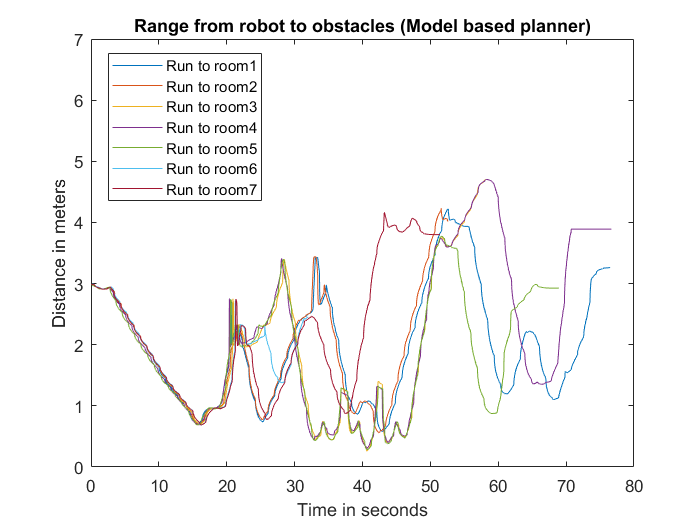
\includegraphics[width=0.95\textwidth]{PlotModelBasedObstacle}
    \caption{Illustration of the distance to the closest obstacle for room 1-7 for the model based planner}
    \label{fig:Model1}
  \end{subfigure}
  \hfill
  \begin{subfigure}[b]{0.49\textwidth}
    \centering
    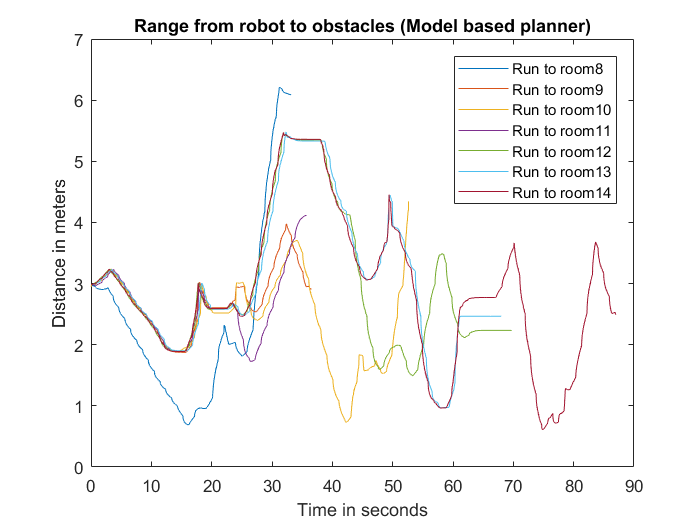
\includegraphics[width=0.95\textwidth]{Plot1ModelBasedObstacle}
    \caption{Illustration of the distance to the closest obstacle for room 8-14 for the model based planner}
    \label{fig:Model2}
  \end{subfigure}
  \hfill
  \begin{subfigure}[b]{0.99\textwidth}
    \centering
    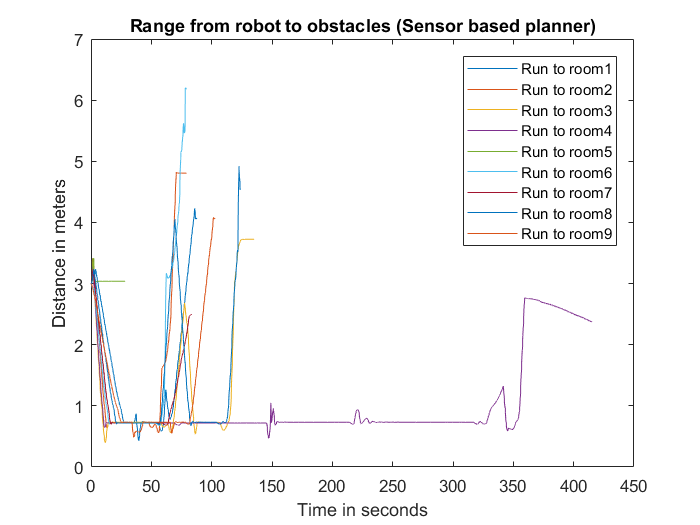
\includegraphics[width=0.47\textwidth]{PlotSensorBasedObstacle}
    \caption{Illustration of the distance to the closest obstacle for room 1-14 for the sensor based planner}
    \label{fig:Sensor 1}
  \end{subfigure}
  \caption{Illustration of the distance to the closest obstacle for room 1-14 for both planners}
\end{figure}
\begin{figure}[H]
  \begin{subfigure}[b]{0.49\textwidth}
    \centering
    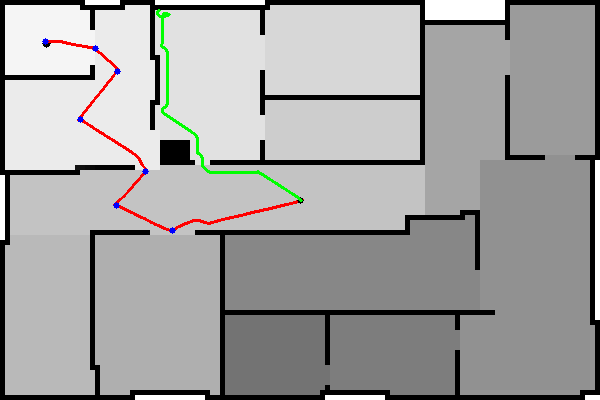
\includegraphics[width=0.9\textwidth]{brushfireAndBugTest1}
    \caption{Illustration of the run from the origin to room 1}
    \label{fig:Test1}
  \end{subfigure}
  \hfill
  \begin{subfigure}[b]{0.49\textwidth}
    \centering
    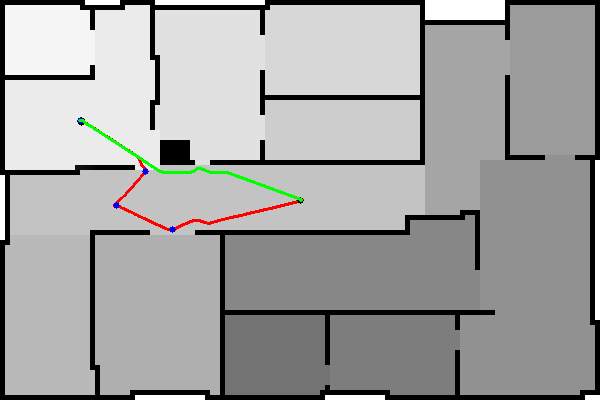
\includegraphics[width=0.9\textwidth]{brushfireAndBugTest2}
    \caption{Illustration of the run from the origin to room 2}
    \label{fig:Test2}
  \end{subfigure}
  \hfill
  \begin{subfigure}[b]{0.49\textwidth}
    \centering
    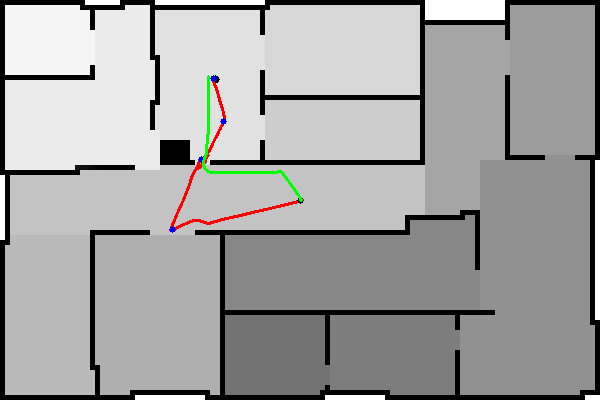
\includegraphics[width=0.9\textwidth]{brushfireAndBugTest3}
    \caption{Illustration of the run from the origin to room 3}
    \label{fig:Test3}
  \end{subfigure}
  \hfill
  \begin{subfigure}[b]{0.49\textwidth}
    \centering
    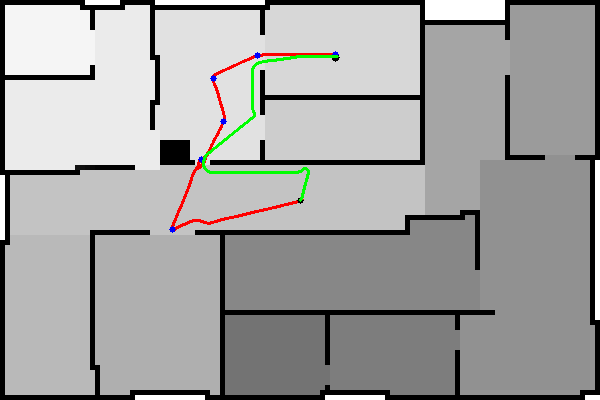
\includegraphics[width=0.9\textwidth]{brushfireAndBugTest4}
    \caption{Illustration of the run from the origin to room 4}
    \label{fig:Test4}
  \end{subfigure}
  \hfill
  \begin{subfigure}[b]{0.49\textwidth}
    \centering
    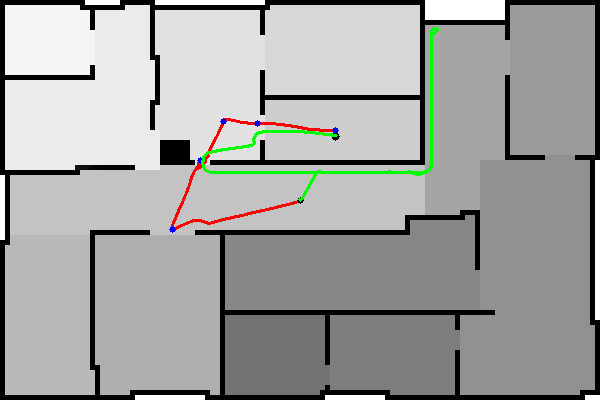
\includegraphics[width=0.9\textwidth]{brushfireAndBugTest5}
    \caption{Illustration of the run from the origin to room 5}
    \label{fig:Test5}
  \end{subfigure}
  \hfill
  \begin{subfigure}[b]{0.49\textwidth}
    \centering
    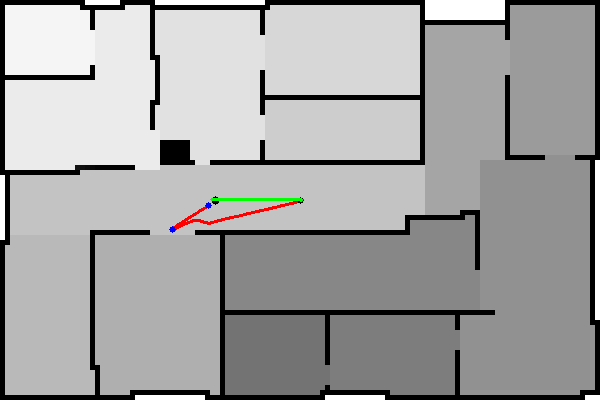
\includegraphics[width=0.9\textwidth]{brushfireAndBugTest6}
    \caption{Illustration of the run from the origin to room 6}
    \label{fig:Test6}
  \end{subfigure}
  \hfill
  \begin{subfigure}[b]{0.49\textwidth}
    \centering
    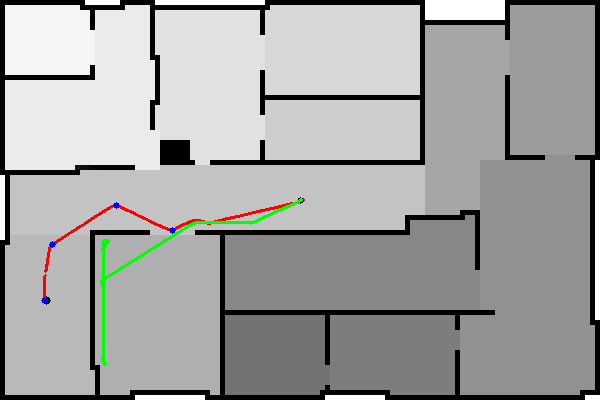
\includegraphics[width=0.9\textwidth]{brushfireAndBugTest7}
    \caption{Illustration of the run from the origin to room 7}
    \label{fig:Test7}
  \end{subfigure}
  \begin{subfigure}[b]{0.49\textwidth}
    \centering
    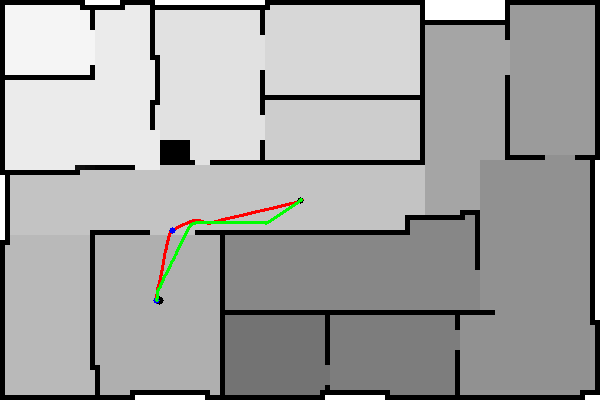
\includegraphics[width=0.9\textwidth]{brushfireAndBugTest8}
    \caption{Illustration of the run from the origin to room 8}
    \label{fig:Test8}
  \end{subfigure}
  \caption{Illustration of the run from the origin to room 1-8 for both the model based (red line) and the sensor based (green line)}
\end{figure}
\begin{figure}[H]
  \begin{subfigure}[b]{0.49\textwidth}
    \centering
    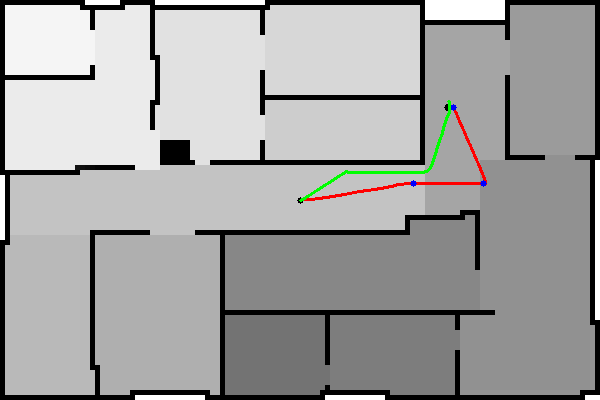
\includegraphics[width=0.9\textwidth]{brushfireAndBugTest9}
    \caption{Illustration of the run from the origin to room 9}
    \label{fig:Test9}
  \end{subfigure}
  \hfill
  \begin{subfigure}[b]{0.49\textwidth}
    \centering
    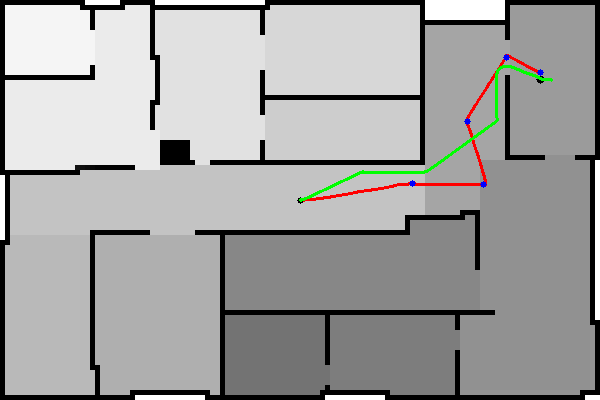
\includegraphics[width=0.9\textwidth]{brushfireAndBugTest10}
    \caption{Illustration of the run from the origin to room 10}
    \label{fig:Test10}
  \end{subfigure}
  \hfill
  \begin{subfigure}[b]{0.49\textwidth}
    \centering
    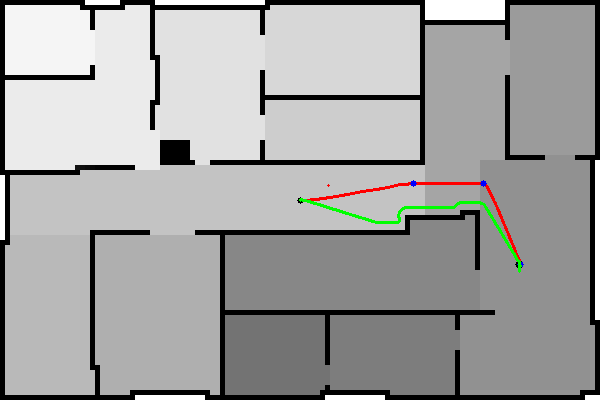
\includegraphics[width=0.9\textwidth]{brushfireAndBugTest11}
    \caption{Illustration of the run from the origin to room 11}
    \label{fig:Test11}
  \end{subfigure}
  \hfill
  \begin{subfigure}[b]{0.49\textwidth}
    \centering
    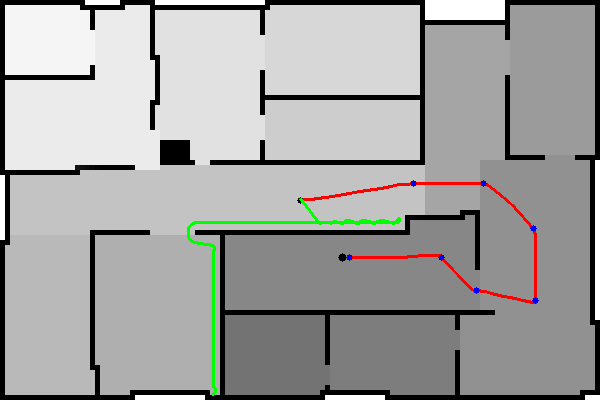
\includegraphics[width=0.9\textwidth]{brushfireAndBugTest12}
    \caption{Illustration of the run from the origin to room 12}
    \label{fig:Test12}
  \end{subfigure}
  \begin{subfigure}[b]{0.49\textwidth}
    \centering
    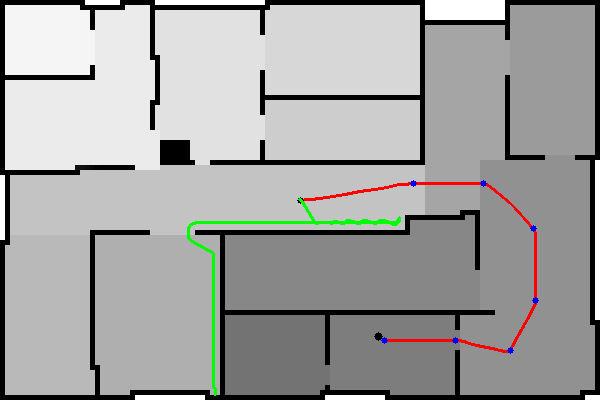
\includegraphics[width=0.9\textwidth]{brushfireAndBugTest13}
    \caption{Illustration of the run from the origin to room 13}
    \label{fig:Test13}
  \end{subfigure}
  \hfill
  \begin{subfigure}[b]{0.49\textwidth}
    \centering
    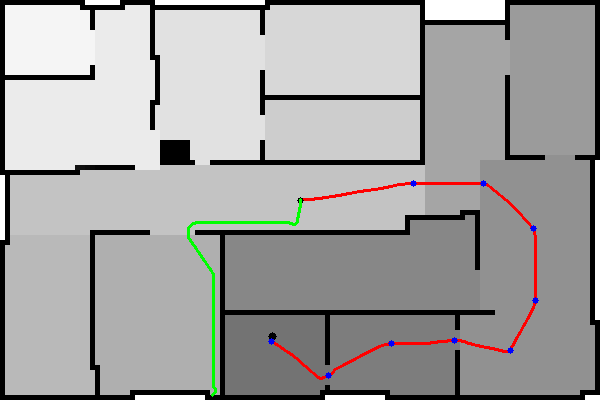
\includegraphics[width=0.9\textwidth]{brushfireAndBugTest14}
    \caption{Illustration of the run from the origin to room 14}
    \label{fig:Test14}
  \end{subfigure}
  \caption{Illustration of the run from the origin to room 9-14 for both the model based (red line) and the sensor based (green line)}
\end{figure}
\begin{figure}[H]
	\centering
	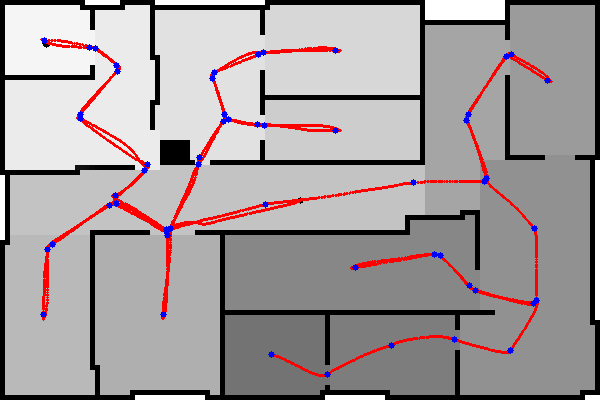
\includegraphics[width=0.6\textwidth]{brushfireTest15}
	\caption{Illustration of the run visiting all rooms starting from the origin for the model based planner}
	\label{fig:Test15}
\end{figure}
\end{document}